\documentclass[a4paper,11pt]{ltjsarticle}
\usepackage[top=24mm,bottom=24mm,left=24mm,right=24mm,headheight=16pt]{geometry}
\usepackage{luatexja-fontspec}
\setmainjfont{Noto Serif CJK JP}\setsansjfont{Noto Sans CJK JP}
\setmainfont{DejaVu Serif}\setsansfont{DejaVu Sans}\setmonofont{DejaVu Sans Mono}[Scale=.82]
\usepackage{amsmath,amssymb,amsthm,mathtools,bm}
\usepackage{booktabs,longtable,tabularx,array,graphicx,caption,float}
\usepackage{fancyhdr,enumitem,listings,xurl}
\usepackage[unicode,hidelinks]{hyperref}
\hypersetup{pdftitle={境界を保つRGB-Dシーンフロー補正：頑健な幾何項・剛体補助項・高速数値解法},pdfauthor={Technical research report}}
\setlength{\parindent}{1em}\setlength{\parskip}{.3em}\setlength{\emergencystretch}{3em}
\linespread{1.06}\setlist{nosep,leftmargin=1.7em}
\captionsetup{font=small,labelfont=bf,labelsep=quad}
\pagestyle{fancy}\fancyhf{}\fancyhead[L]{\small 境界を保つRGB-Dシーンフロー補正}\fancyhead[R]{\small 第0.3版}\fancyfoot[C]{\thepage}
\newcommand{\R}{\mathbb R}\newcommand{\T}{\mathsf T}\newcommand{\norm}[1]{\left\lVert#1\right\rVert}
\newcommand{\abs}[1]{\left|#1\right|}\newcommand{\argmin}{\operatorname*{arg\,min}}
\newcommand{\prox}{\operatorname{prox}}\newcommand{\clip}{\operatorname{clip}}\newcommand{\proj}{\operatorname{proj}}
\newcommand{\diag}{\operatorname{diag}}\newcommand{\SO}{\operatorname{SO}}\newcommand{\med}{\operatorname{med}}
\newcommand{\Reg}{\mathcal R}\newcommand{\NA}{---}\newcommand{\code}[1]{\texttt{\detokenize{#1}}}
\theoremstyle{definition}
\newtheorem{definition}{定義}[section]\newtheorem{assumption}[definition]{仮定}
\newtheorem{proposition}[definition]{命題}\newtheorem{remark}[definition]{注意}
\renewcommand{\proofname}{証明}
\lstset{basicstyle=\ttfamily\footnotesize,breaklines=true,columns=fullflexible,keepspaces=true,frame=single}
\newcommand{\HeldOld}{2.804}
\newcommand{\HeldNew}{0.991}
\newcommand{\HeldTimeOld}{34.946}
\newcommand{\HeldTimeNew}{9.890}

\begin{document}
\hypersetup{pageanchor=false}
\begin{titlepage}
\vspace*{10mm}
{\sffamily\large 理論仕様・数値解法・再現可能な比較実験}\par\vspace{10mm}
{\sffamily\huge 境界を保つ\par RGB-Dシーンフロー補正}\par\vspace{5mm}
{\sffamily\Large 頑健な幾何項・剛体補助項・高速数値解法}\par\vspace{9mm}
第0.3版\quad 2026年10月13日\par\vspace{8mm}
\hrule\vspace{6mm}
\textbf{要旨}\par
深度と灰度画像から得た初期フローの誤差を、有限候補の再探索と境界を保つ二階正則化で補正します。
前版に対し、対応探索の階層化、計算の融合、双対変数の再利用、
幾何残差に対するベクトルHuber損失、観測だけから推定する剛体運動の補助項を追加しました。
物理的な移動上限は維持し、補助項の寄与は有限の重みに限定します。

主比較は、前版と同じ6入力の再試験と、形状・姿勢・模様・運動を変えた新規6入力で分離しています。
新規入力での平均3次元端点誤差は前版\HeldOld{} mm、標準版\HeldNew{} mm、
平均C++処理時間は\HeldTimeOld{}秒、\HeldTimeNew{}秒でした。
単一要素の除去に加え、Huber化と剛体補助項の$2\times2$比較を実施しています。

本方式は、全シーンが剛体であることを保証しません。深度連結領域が異なる運動を含む場合、
補助項は有害になり得ます。深度欠測の完全な補完、観測できない球の回転の復元、
実時間動作、実データへの一般化、全非凸問題の大域最適性は主張しません。
\vfill
\small
実装：C++17・倍精度・CPU単一スレッド\par
環境：uv / Python\quad 文書：LuaLaTeX\par
固定条件の数式、証明、コードとの対応、実験条件、失敗例を本文内で定義します。
\end{titlepage}
\pagenumbering{roman}\hypersetup{pageanchor=true}
\setcounter{tocdepth}{2}\tableofcontents\clearpage\pagenumbering{arabic}

\section{問題設定と今回の結論の範囲}
\subsection{何を改善するか}
既存の第0.2版は、球・立方体・円柱・楕円体、動く影、遮蔽を含む人工データに対して、
初期フローと両時刻の深度を補正するC++実装です。
本版の比較基準はこの第0.2版であり、それ以前の平面中心の第0.1版ではありません。
異なる人工データの誤差を並べて精度向上とみなすことも避けます。

前版の代表入力の再計測は約34.5秒で、うち約19.1秒を対応探索が占めました。
探索は往復の広域探索と、多数の小数画素候補の評価を行い、各候補で一時配列を確保していました。
最適化は主双対法で、外側の反復ごとに双対変数をゼロへ戻していました。
一方、行列の行・列絶対和による対角前処理は既に実装済みでした。
従って、\textbf{対角前処理を今回初めて導入したという説明はしません。}

精度上の主要な問題は、影などに整合した誤対応が二乗の幾何項で強く維持されることと、
画像座標上の滑らかさだけでは、曲面上の回転や遮蔽部の運動を十分に拘束できないことです。
ただし、後者を剛体モデルで補うと、モデルに適合しない運動に偏りが生じます。
これを実験上の独立した仮説として扱います。

\subsection{文献調査から採用したもの・採用しなかったもの}
\begingroup\small
\begin{longtable}{p{.26\linewidth}p{.66\linewidth}}
\toprule 文献・資料 & 今回の扱い\\\midrule\endhead
YaoらのB-ADT\cite{yao} & 境界を横切る正則化を停止する考え方を継承します。原論文の逆深度補完法や標準TGVの忠実な移植ではありません。\\
DIS\cite{dis} & 初期フローを灰度画像から推定する比較基準として維持します。今回の候補縮小は独自の有限探索であり、DISの逆合成法の再実装ではありません。\\
UnFlow\cite{unflow} & 照明変化と往復整合の重要性を参考にします。Censusや学習ネットワークは追加せず、局所輝度の利得補正を別条件で検証します。\\
区分剛体モデル\cite{vogel} & 複数の剛体運動で対応を補助する発想を参考にします。本版は深度連結領域で事前推定した固定補助項であり、元論文の領域分割最適化ではありません。\\
Horn\cite{horn} & 単位四元数による重み付き剛体当てはめを実装します。尺度は1に固定し、Huber重みの反復で外れ値の影響を抑えます。\\
対角前処理\cite{pock,naganuma} & 前処理の収束条件と、ブロック内で等しい計量を用いる意味を確認します。本版の単純なノルム評価は本文で証明します。\\
IEEE執筆指針・NeurIPS検査項目\cite{ieee,checklist} & 記号の初出定義、仮定と結論の分離、図表の単位、再現条件、誤差棒の意味、失敗条件を明記します。投稿様式をそのまま模倣するものではありません。\\\bottomrule
\end{longtable}
\endgroup

\subsection{比較資料の範囲}
共有済みZIPと保存配列を使用しました。追加の「他エージェントの実験結果」は、
本実行時に読める本文・添付として確認できなかったため、比較表に含めていません。
存在が確認できない測定値を採用したり、他エージェントによる独立検証として数えたりしていません。

\section{座標、観測、未知量}
\subsection{入力契約}
\begin{assumption}[標準設定の適用域]\label{ass:domain}
2時刻でカメラは固定され、灰度画像と深度画像は同じ画素格子に位置合わせ済みです。
内部パラメータは既知で、深度は光軸方向の距離です。
物体点の時刻間変位の上限$\delta$は$0<\delta<d_{\min}$を満たします。
欠測以外の観測深度は$[d_{\min},d_{\max}]$内にあり、両時刻で同じ単位を用います。
\end{assumption}
画素領域は$\Omega=\{0,\ldots,W-1\}\times\{0,\ldots,H-1\}$、$N=HW$です。
整数座標は画素中心を表します。画像の$x,y$は右・下、カメラ座標$X,Y,Z$は右・下・前です。
長さはメートル、フローは画素単位です。未知量$S$は変位であり、時間差で割った速度ではありません。
\begin{center}\small
\begin{tabularx}{\linewidth}{lX}\toprule 記号 & 定義\\\midrule
$I_t:\Omega\to[0,1]$ & 時刻$t\in\{0,1\}$の観測灰度画像\\
$\widehat d_t,\ M_t$ & 観測深度、および有限かつ正の観測の画素集合\\
$\widehat f_p\in\R^2$ & 外部で推定した時刻0から1へのフロー\\
$d_t:\Omega\to\R,\ S_p\in\R^3$ & 補正する深度場、各画素の3次元変位\\
$r(p)$ & $((p_x-c_x)/f_x,(p_y-c_y)/f_y,1)^\T$\\
$\pi(X)$ & $(f_xX_x/X_z+c_x,f_yX_y/X_z+c_y)$、$X_z>0$\\
$\mathcal C_p,\ k_p$ & 有限の対応候補集合、その選択番号\\
$m_p\in\{0,1\}$ & 前処理で決める対応支持。真の可視性ではありません\\
$\mu_p,\beta_p$ & 観測から求める固定の剛体変位予測と補助重み\\
$\ell,\ z_t=d_t/\ell,\ s=S/\ell$ & 数値計算用の長さ尺度と無次元変数\\\bottomrule
\end{tabularx}\end{center}
標準値は$\ell=0.01$ m、$d_{\min}=0.1$ m、$d_{\max}=5$ m、$\delta=0.05$ mです。
RGB入力も許容しますが、今回の実験は同じ灰度を三成分へ複製した入力です。
三成分の一致をC++側で検出し、同一の残差を三回計算しないようにしました。

\subsection{補正許容域と幾何}
有効な深度観測には、次の閉区間を与えます。
\begin{equation}\label{eq:box}
B_t(p)=[d_{\min},d_{\max}]\cap
[\widehat d_t(p)-\kappa\sigma_d,\ \widehat d_t(p)+\kappa\sigma_d].
\end{equation}
$p\notin M_t$なら$B_t(p)=[d_{\min},d_{\max}]$です。標準は$\kappa=4$、$\sigma_d=0.003$ mです。
この区間は観測の確率的な信頼区間として校正したものではなく、許す補正量の仕様です。

候補$q_p^k$を囲む最大4画素の添字を$j_{pkh}$、双一次重みを$a_{pkh}\ge0$とし、
$\sum_h a_{pkh}=1$とします。潜在深度の幾何式には4係数をそのまま用います。
一方、観測深度の支持判定・観測値の補間では、$\mathcal H_{pk}=\{h:a_{pkh}>10^{-14}\}$だけを使用します。
この数値規則は欠測値と0の積を避けるためのもので、残る重みを再規格化しません。
$\bar z_{1,p}^{k}=\sum_h a_{pkh}z_1(j_{pkh})$と置くと、無次元の幾何残差は
\begin{equation}\label{eq:geometry}
g_p(x,k_p)=\bar z_{1,p}^{k_p}r(q_p^{k_p})-z_0(p)r(p)-s_p
\end{equation}
です。$k$を固定すれば未知量に対して線形です。対応先の深度画像は全画素で共有し、
対応ごとに別の深度変数を作りません。
出力フローは、選択候補のフローと再投影フローを区別します。
\begin{equation}\label{eq:flows}
f_p^{\mathrm{match}}=q_p^{k_p}-p,\qquad
f_p^{\mathrm{proj}}=\pi(d_0(p)r(p)+S_p)-p.
\end{equation}
幾何整合性を柔らかい損失で表すため、両者は一般に一致しません。

\section{観測だけによる有限候補の生成}
\subsection{深度誤差を許した物理的な除外}
候補の補間支持に欠測がある場合、または支持内の観測深度差が$\theta_e=0.06$ mを超える場合は、
その候補を除きます。深度境界を混ぜた中間面を作らないための保守的な規則です。
その後、式\eqref{eq:box}から得る二つの光線区間間の距離が$\delta$を超える候補を除きます。
\begin{equation}\label{eq:gate}
\min_{a\in[l_0,u_0],\ b\in[l_1,u_1]}
\norm{b r(q)-a r(p)}_2\le\delta.
\end{equation}
$[l_1,u_1]$は対応先の各深度区間の端点を、非負の双一次重みで加重した区間です。
厳密な係数による式は必要条件です。実装では$\mathcal H_{pk}$だけを加重し、距離検査に$10^{-12}$ mの許容を加えます。
従って数値実装まで厳密な実数演算の必要条件判定とは呼びません。
この検査は\textbf{候補ごとの必要条件}であって、画像全体で同じ深度場を共有する全対応が
同時に厳密整合できることを保証しません。

\begin{proposition}[光線区間距離の有限評価]
$r_0,r_1$の$Z$成分を1、$l_t>0$とします。
$A=r_0^\T r_0$、$B=r_0^\T r_1$、$C=r_1^\T r_1$とすると、
式\eqref{eq:gate}の最小値は、$a=l_0,u_0$に対して
$b=\clip(aB/C,l_1,u_1)$を評価し、$b=l_1,u_1$に対して
$a=\clip(bB/A,l_0,u_0)$を評価した、四つの候補の最小値です。
\end{proposition}
\begin{proof}
二乗距離は$Aa^2-2Bab+Cb^2$です。片方を固定した最小化は1変数の凸二次式の射影です。
二つの光線が非平行なら、内部の停留点は$a=b=0$だけであり、正の区間内にはありません。
従って最小点は長方形の辺上にあります。平行なら光線方向が等しく、区間の重なりがある場合も
いずれかの辺の射影で距離0を得られます。重なりがない場合も辺の評価で最小値を得ます。
\end{proof}

\subsection{照合コストと照明差}
$p$と候補$q$の周囲の同じオフセットで、深度段差をまたがずに灰度を取得できる組の集合を
$P(p,q)$とします。半径2の$5\times5$窓を用い、平均除去時には少なくとも3組を要求します。
各組の灰度を$u_i,v_i$、その平均を$\bar u,\bar v$と置きます。
Huber損失を
\begin{equation}\label{eq:huber}
h_k(a)=\begin{cases}\frac12a^2,&|a|\le k,\\ k(|a|-\frac12k),&|a|>k\end{cases}
\end{equation}
と定義し、標準の画像コストは
\begin{equation}\label{eq:photo}
C_I(p,q)=\frac{1}{|P(p,q)|}\sum_{i\in P(p,q)}
h_2\!\left(\frac{v_i-u_i-(\bar v-\bar u)}{\sigma_I}\right),\quad \sigma_I=0.025
\end{equation}
です。平均除去は加算的な輝度差を除きますが、影の境界や模様の不在まで解消するものではありません。

アブレーションで試す利得補正は、次の制限付き最小二乗の係数を先に求め、
式\eqref{eq:photo}の残差を$v_i-a u_i-b$へ置き換えます。
\begin{equation}\label{eq:gain}
a=\clip\!\left(\frac{\sum_i(u_i-\bar u)(v_i-\bar v)}{\sum_i(u_i-\bar u)^2},\frac12,2\right),
\qquad b=\bar v-a\bar u.
\end{equation}
分母が$10^{-10}$以下なら$a=1$です。
係数は二乗誤差で求め、評価はHuber損失で行う\textbf{代入型の記述子}です。
Huber損失について$a,b$も厳密に同時最小化しているとは記述しません。
標準版では利得補正を無効にし、有効時の効果を独立に測定します。

候補の固定コストは
\begin{equation}\label{eq:cost}
C_p(k)=\lambda_I C_I(p,q_p^k)+\lambda_f
\min\!\left(\frac{\norm{q_p^k-p-\widehat f_p}^2}{2\sigma_f^2},\tau_f\right)
\end{equation}
です。$\lambda_I=1$、$\lambda_f=0.025$、$\sigma_f=0.7$画素、$\tau_f=9$を用います。
非有限の初期フローでは、フロー観測項を切断値に置きます。

\subsection{候補を減らす方法と限界}
$z_0\ge l_0$、$\norm{S}\le\delta$なら、横方向の投影変位には
\begin{equation}\label{eq:radius}
|f_x|\le\frac{f_x^{\mathrm{cam}}\delta\sqrt{1+r_x(p)^2}}{l_0-\delta}
\end{equation}
という上界が成立し、縦方向も同様です。ここだけ$f_x^{\mathrm{cam}}$は焦点距離を表します。
分子は$S_x-r_xS_z$へのCauchy--Schwarz不等式、分母は正の下界から得ます。
この範囲を丸めて1画素の余裕を加え、計算上の最大半径18画素で制限します。

第0.2版の整数画素全探索と、多数の$1/8$画素候補の評価を、標準版では次の有限規則に置き換えます。
整数候補を2画素間隔で走査し、恒等対応と観測フローの対応を加えます。
観測コスト順に、原則1.5画素以上離れた最大3個の種を選びます。
各種の周囲を刻み$1/2,1/4,1/8$画素の順に$3\times3$で探索し、各段の最良点へ中心を移します。
各段の中心以外の8点を評価します。
候補をコストで整列し、まず0.65画素以上離れた候補を最大12個、次に0.04画素未満の重複を除いて最大24個を保持します。
恒等対応が得られ、まだ保持されていない場合は、最後の候補と置き換えて保持します。
恒等対応を選ぶことを強制する規則ではありません。

候補最良点の$C_I\le3$を要求し、逆向きにも同様の探索を行います。
逆向きはフロー観測重みを0にし、再帰的な往復検査は行いません。
往復差が1.5画素を超える点、または逆向き補間の有効重みが0.99未満の点は$m_p=0$とします。
$m$は以後固定します。後の候補更新のたびに可視性を再推定する方式ではありません。

探索の階層化と最大半径は近似です。連続領域の最良対応、あるいは全ての物理的に可能な対応が
保持されるという保証はありません。各対応候補には観測だけを用い、正解フローは使いません。

\section{固定する剛体運動の補助項}
\subsection{深度連結領域と頑健な当てはめ}
時刻0の有効深度画素を4近傍で結び、隣接観測深度差が$\theta_e$以下の辺だけを残します。
その連結成分を$\Gamma_\nu$と呼び、$\nu=0,\ldots,G_\Gamma-1$を領域番号、$G_\Gamma$を領域数とします。これは\textbf{物体の正解領域ではありません}。
接している別物体、滑らかにつながる床と壁などを同じ領域へまとめることがあります。

$m_p=1$の画素で、最初の最良候補$k_p=0$から観測点対を作ります。
\begin{equation}
\widehat X_p=\widehat d_0(p)r(p),\qquad
\widehat Y_p=\left(\sum_{h\in\mathcal H_{p0}} a_{p0h}\widehat d_1(j_{p0h})\right)r(q_p^0),\qquad
b_p=(1+C_I(p,q_p^0))^{-1}.
\end{equation}
各領域内で、尺度1の剛体変換を次の頑健な目的で当てはめます。
\begin{equation}\label{eq:fit}
\min_{Q\in\SO(3),\ t\in\R^3}
\sum_{p\in\Gamma_\nu:m_p=1} b_p\,
 h_1\!\left(\frac{\norm{Q\widehat X_p+t-\widehat Y_p}}{h_R}\right),
\quad h_R=0.006\ \mathrm m.
\end{equation}
初期重みを$b_p$とし、重み付き剛体最小二乗と
$\omega_p=b_p\min(1,h_R/\max(10^{-12},\norm{e_p^R}))$の更新を8回行います。ここで$e_p^R=Q\widehat X_p+t-\widehat Y_p$は剛体当てはめの残差です。
重み付き最小二乗はHorn法\cite{horn}で解きます。\eqref{eq:fit}の大域最小化や8回での収束を保証しません。

採用条件は、有効点対が24点以上かつ領域の10\%以上であること、
点対の出発点の無重み共分散について二次主小行列式の和が$10^{-10}\ \mathrm m^4$以上であること、
最終残差の上側中央値$\widetilde e_\nu$が$1.5h_R$以下であることです。
共分散条件は、点状・ほぼ直線状の支持を除く簡易検査です。
偶数個の場合の上側中央値は、昇順の$\lfloor n/2\rfloor+1$番目とします。

\subsection{補助項の意味を限定します}
採用領域では、観測時点の点に対する予測を固定します。
\begin{equation}\label{eq:prior}
\mu_p=(Q_\nu-I)\widehat X_p+t_\nu,\qquad
\beta_p=\min\!\left(1,\frac{h_R^2}{\max(10^{-12},\widetilde e_\nu^2)}\right).
\end{equation}
採用しない領域・深度欠測点では$\beta_p=0$です。推定する$S$に対し、
$\beta_p\norm{S_p-\mu_p}^2/(2\sigma_R^2)$という有限の罰則を加えます。
標準値は$\sigma_R=0.0015$ mです。

$\mu$は未知深度$d_0$ではなく、観測深度$\widehat d_0$から作った固定予測です。
従って本版は姿勢と潜在深度を完全に同時推定する方式ではありません。
また、同じ観測を照合にも補助項にも用いるため、
\textbf{独立な事前分布と尤度を掛け合わせた校正済みのベイズ推定とは解釈しません}。
$\beta$も可視性の確率や正答確率ではなく、経験的な重みです。

画素上の二階正則化は、$S(p)$が画素座標に対してほぼ一次であることを好みます。
一方、剛体運動は$S(X)=(Q-I)X+t$であり、3次元位置に対して一次です。
曲面では$X(p)$が一次でないため、この違いが補助項を用いる理由です。
ただし、柔らかい補助項を加えた出力自体が厳密な剛体運動になるわけではありません。

\section{全目的関数と離散演算子}
\subsection{境界を保つ二階正則化}
時刻$t$の観測深度で定まる有向の右・下隣接辺集合を$E_t$とします。
端点のいずれかが欠測、または深度差が$\theta_e$を超える辺は含めません。
$c$成分の場$u_p\in\R^c$に、補助場$w_p\in\R^{2\times c}$を導入します。
辺$e=(p,r,a)$の方向$a\in\{x,y\}$について
\begin{equation}\label{eq:regularizer}
\Reg_E(u,w)=\alpha_1\sum_{(p,r,a)\in E}
 \norm{u_r-u_p-\tfrac12(w_{p,a}+w_{r,a})}_2
 +\alpha_0\sum_{(p,r,a)\in E}\norm{w_r-w_p}_F
\end{equation}
とします。画像外への差分は作りません。境界を横切る辺は\textbf{両項から}除きます。
これは全勾配型のグラフ二階正則化です。標準的な対称勾配TGVと同一ではありません。
一次TV比較では補助場を差分から除き、第一項を$\alpha_1\sum_E\norm{u_r-u_p}$に置き換えます。

$A\in\R^{c\times2}$に対して$u(p)=Ap+b$、$w=A^\T$なら、\eqref{eq:regularizer}の半ノルム部分は0です。
後述の小さな二次罰則を含めた全正則化まで0になる、という意味ではありません。
離散画素間隔は数値上1とします。解像度を変えても同じ$\alpha$を使うことは、
同じ連続体の正則化を厳密に再現する尺度変換ではありません。

\subsection{標準版の定義}
$\eta_d=\sigma_d/\ell$、$\eta_g=\sigma_g/\ell$、$\eta_R=\sigma_R/\ell$、
$\widetilde\mu=\mu/\ell$とします。$\sigma_g=0.0008$ m、$k_d=k_g=3$です。
$\Reg_d,\Reg_s$にはそれぞれ深度用・変位用の係数を使います。
未知ベクトルの順序を
\[
x=(z_0,z_1,s,w_0,w_1,w_s)\in\R^{15N}
\]
と固定し、以下を本版の最適化問題と定義します。
\begin{equation}\label{eq:objective}
\begin{split}
\min_{x,k}\quad &
 \sum_{t=0}^{1}\sum_{p\in M_t}
 h_{k_d}\!\left(\frac{z_t(p)-\widehat d_t(p)/\ell}{\eta_d}\right)\\
 &+\sum_{p:m_p=1}\left[C_p(k_p)+
 h_{k_g}\!\left(\frac{\norm{g_p(x,k_p)}}{\eta_g}\right)\right]\\
 &+\Reg_d(z_0,w_0;E_0)+\Reg_d(z_1,w_1;E_1)
    +\Reg_s(s,w_s;E_0)\\
 &+\frac{1}{2\eta_R^2}\sum_p\beta_p\norm{s_p-\widetilde\mu_p}^2
   +\frac{\varepsilon}{2}\left(\norm{w_0}^2+\norm{w_1}^2+\norm{w_s}^2\right),\\
\text{条件}\quad & z_t(p)\in B_t(p)/\ell,\qquad
 \norm{s_p}\le\delta/\ell,\qquad k_p\in\mathcal C_p\ (m_p=1).
\end{split}
\end{equation}
$\varepsilon=10^{-6}>0$です。$m_p=0$の点では$k_p$を必要とせず、対応の項はありません。
その点の変位は空間的な正則化や、採用された補助項で決まります。
各深度観測のデータ項は一度だけ評価します。

幾何項のHuber化を外す比較では、$h_{k_g}(\norm{g}/\eta_g)$を$\norm{g}^2/(2\eta_g^2)$に変更します。
切断型の非凸損失ではなく、凸なHuber損失を選んだため、固定対応の部分問題の凸性を保ちます。
移動上限を満たすために、最適化終了後の3次元ベクトルだけを切り詰める手順は採用しません。

\begin{proposition}[解の存在と固定対応の凸性]\label{prop:convex}
仮定\ref{ass:domain}を満たし、候補、支持、境界、$\mu,\beta$を固定します。
各有効点の候補集合は有限で空でないとします。
式\eqref{eq:objective}は最小値を持ちます。$k$を固定した部分問題は凸です。
ただし、解の一意性や、$k$を含む問題全体の凸性は主張しません。
\end{proposition}
\begin{proof}
深度区間と変位球は非空のコンパクトな凸集合です。
$k$を固定すれば$g$と正則化の差分は線形で、
非減少な凸関数$h_{k_g}$とノルムの合成は凸です。他の項も凸です。
正の$\varepsilon$により、有限の目的値の部分集合上で補助場$w$は有界です。
目的は連続、制約集合は閉なので、有限次元のコンパクトな部分集合上で最小値が達成されます。
各$k$の組合せは有限個であり、その最小値の最小を取れば全問題の最小値も達成されます。
この存在証明は、その解を実際の反復で発見できることを意味しません。
\end{proof}

\section{数値解法と保証}
\subsection{外側の候補更新}
候補、支持、境界、補助項は前処理後に固定します。最初は各画素の最良観測候補を選びます。
深度は観測値、欠測は許容域内の1 mで初期化し、支持点の変位は最初の候補の逆投影で初期化します。
移動球へ射影し、無支持点の変位と補助場は0にします。
外側の2回目以降には、現在の$x$について各画素独立に
\begin{equation}\label{eq:discrete_update}
k_p\leftarrow\argmin_{k\in\mathcal C_p}
 \left[C_p(k)+h_{k_g}(\norm{g_p(x,k)}/\eta_g)\right]
\end{equation}
を厳密に全列挙します。同値の場合は保持順の先頭を選びます。
その後、固定対応の凸問題を主双対法で所定回数解きます。

\subsection{行列分割と対角前処理}
固定対応の問題を$\min_x G(x)+F(Kx)$と書きます。
$G$は深度観測項、区間制約、移動球、剛体補助項、小さな二次罰則です。
$K$は式\eqref{eq:regularizer}の二つの差分と式\eqref{eq:geometry}を並べた疎行列で、
$F$は各グループのノルムまたはHuber損失です。候補コストは固定定数です。
CSR形式で$K$を保存し、転置積は同じ非零要素を使って足し戻します。

$A_i=\sum_j|K_{ij}|$、$B_j=\sum_i|K_{ij}|$、$\theta=0.95$とし、
まず$T_{jj}=\theta/\max(1,B_j)$、$\Sigma_{ii}=\theta/\max(1,A_i)$とします。
各変位の3成分では$T$をその最小値に揃え、各双対ノルムのグループでも$\Sigma$を最小値に揃えます。
これにより、球への近接写像を単純なユークリッド射影で計算できます\cite{naganuma}。
任意の固定$\chi>0$について$T\leftarrow\chi T$、$\Sigma\leftarrow\Sigma/\chi$としても
以下のノルム条件は変わりません。標準は$\chi=1$です。

\begin{proposition}[前処理の安全な上界]\label{prop:steps}
この構成は$\norm{\Sigma^{1/2}KT^{1/2}}_2\le\theta<1$を満たします。
\end{proposition}
\begin{proof}
任意の$v$に対し、重み付きCauchy--Schwarz不等式から
\begin{align*}
\norm{\Sigma^{1/2}KT^{1/2}v}^2
 &\le\sum_i\Sigma_{ii}A_i\sum_j |K_{ij}|T_{jj}v_j^2\\
 &\le\theta\sum_j B_jT_{jj}v_j^2\le\theta^2\norm{v}^2.
\end{align*}
ブロック内でステップを小さく揃える操作は不等式を壊しません。
$T,\Sigma$の相反する定数倍も積を変えません。
\end{proof}
出力の\code{operator_norm_bound}は0.95という\textbf{証明上の上界}であり、
実際の最大特異値を計測した値ではありません。前処理の文献上の背景は\cite{pock,naganuma}です。

\subsection{主双対更新と近接写像}
$\bar x^0=x^0$として、反復は
\begin{equation}\label{eq:pdhg}
\begin{split}
y^{n+1}&=\prox_{F^*}^{\Sigma^{-1}}(y^n+\Sigma K\bar x^n),\\
x^{n+1}&=\prox_G^{T^{-1}}(x^n-TK^\T y^{n+1}),\\
\bar x^{n+1}&=2x^{n+1}-x^n
\end{split}
\end{equation}
です。上付きの計量は、例えば$\prox_G^{T^{-1}}(v)=
\argmin_u[G(u)+\frac12\norm{u-v}_{T^{-1}}^2]$を意味します。

ノルム群$F_j(v)=\alpha\norm{v}$の双対近接写像は半径$\alpha$の球への射影です。
幾何Huber群は$F_j(v)=m h_{k_g}(\norm{v}/\eta_g)$です。
$m=1$の行だけを作り、$w=m/\eta_g^2$、$c=mk_g/\eta_g$とすると
\begin{equation}\label{eq:dual_huber}
F_j^*(y)=\frac{\norm{y}^2}{2w}+\iota_{\{\norm{y}\le c\}}(y),\quad
\prox_{\sigma F_j^*}(v)=\proj_{\norm{\cdot}\le c}\left(\frac{v}{1+\sigma/w}\right).
\end{equation}
二乗幾何項では球への射影だけを除きます。Huber損失は、大きな幾何残差の影響に上限を与えますが、
残差を完全に無視するものではありません。

深度の近接写像について、入力を$v$、観測を$a$、ステップを$\tau$、尺度を$\eta$とします。
区間制約を除いた差分$u-a$は
\begin{equation}\label{eq:depth_prox}
u-a=\begin{cases}
(v-a)/(1+\tau/\eta^2),&|v-a|\le k(\eta+\tau/\eta),\\
v-a-(\tau k/\eta)\operatorname{sign}(v-a),&\text{それ以外}
\end{cases}
\end{equation}
であり、これを許容区間へ射影します。1変数の凸問題なので、この順序は厳密です。
欠測点は観測項を持たず、区間への射影だけです。

変位の近接写像は、$\zeta_p=\beta_p/\eta_R^2$として
\begin{equation}\label{eq:scene_prox}
s_p=\proj_{\norm{\cdot}\le\delta/\ell}
\left(\frac{v_p+\tau_p\zeta_p\widetilde\mu_p}{1+\tau_p\zeta_p}\right)
\end{equation}
です。3成分に等しいステップを使うため、補助項と球を合わせて正確に処理できます。
補助場の近接写像は成分ごとに$v_j/(1+T_{jj}\varepsilon)$です。

\subsection{融合、再利用、有限反復}
双対更新では、$K\bar x$の計算、双対変数の更新、双対近接写像、$K^\T y$への足し戻しを
同じグループの走査内で実行します。大きな中間配列と複数回のグループ走査を省きます。
行列も目的関数も変えない実装変更です。融合しない参照経路を残し、数値一致を試験します。

外側の反復で行の意味と順序は変わらず、幾何行の係数だけが変わるため、
前ブロックの双対変数を次の初期値として再利用します。これは最適性の保証ではなく初期化です。
標準は外側3回、内側$400+150+150=700$回です。
前版の$600\times3=1800$回との違いは、探索や計算融合の変更と分けて比較します。

25回ごとと最後に目的値を計算し、開始点も含めた最良の主変数と対応する双対変数を保持します。
主双対法の各反復の目的値が単調に減る、という誤った主張はしません。
現在の候補も候補集合に含まれるため、式\eqref{eq:discrete_update}と最良点保持によって、
外側で受理される目的値は丸め誤差を除き増加しません。
固定対応で反復を十分継続する場合の主双対法の収束条件と、
有限回で打ち切る本実装の精度は区別します。

\subsection{残差の意味}
保持した$(x,y)$について、$\bar x=x$として近接写像を一回適用し、
\begin{equation}\label{eq:residual}
r_P=\max_j\frac{|x_j-\prox_G^{T^{-1}}(x-TK^\T y)_j|}{T_{jj}},\quad
r_D=\max_i\frac{|y_i-\prox_{F^*}^{\Sigma^{-1}}(y+\Sigma Kx)_i|}{\Sigma_{ii}}
\end{equation}
を記録します。出力は最後の固定対応ブロックの値です。
両者は無次元変数に関する固定点残差であり、mm単位の誤差でも相対誤差でもありません。
残差が0でなければ停留条件は厳密には満たしていません。
本版は、この残差から解の誤差や大域最適性の証明済み上界を算出していません。

\section{人工データと評価手順}
\subsection{描画と正解の独立性}
基本形状の光線交差をC++で解析的に計算します。
球・楕円体は$\sum_i a_i^2/s_i^2=1$、直方体は$|a_i|\le s_i$、
円柱は$a_x^2+a_z^2\le s_x^2$かつ$|a_y|\le s_y$、壁・床は有限の平面です。
物体座標で交差を求め、正の交差のうちカメラに最も近いものを採用します。
カメラ光線は$r_z=1$なので交差パラメータは光軸深度です。
灰度の模様を物体の局所座標へ固定し、照明、陰影、影を計算します。
深度と物体番号は画素中心の光線で求め、灰度だけを$2\times2$で標本化します。

出発時の表面の材料座標$a$を保存し、時刻1の位置を$X_1=c_1+Q_1a$として正解変位を求めます。
投影先の連続座標に再度光線を飛ばし、物体番号と奥行きが一致する点を可視とします。
画面内判定には$10^{-9}$画素の丸め誤差許容を使い、奥行き一致の許容は$10^{-8}$ mです。
可視・遮蔽・画面外を排反な集合として保存します。

深度には、標準偏差
$0.003[0.65+0.35(z/1.2)^2]$ mの独立雑音と、画像内標準偏差0.7 mmの空間相関雑音を加えます。
相関雑音は標準偏差1.5画素のGaussian平滑化で生成します。
灰度雑音の標準偏差は0.003です。推定器の公称深度誤差は一律3 mmなので、モデル不一致を含みます。
この人工モデルを、実センサの校正済み雑音モデルとは呼びません。

初期フローはOpenCVのDISから得ます\cite{dis}。
設定はMEDIUM、最細レベル0、パッチ8画素、間隔3画素、単一スレッドです。
正解の深度・領域・変位・可視性を推定器へ渡す引数はありません。
正解に誤差を加える既存生成器も残しますが、今回の主比較は全て画像からの初期フローです。

\subsection{開発条件と新規条件の分離}
\begin{center}\small
\begin{tabularx}{\linewidth}{lX}\toprule 区分 & 条件\\\midrule
試作・選択 & 既存の基本配置、雑音種11のみ。探索規則、補助項の強さ、計算回数を検討しました。\\
同一入力の再試験 & 既存の3配置$\times$雑音種11,23。候補やノイズを作り直さず、同じ保存入力へ前版と標準版を適用します。\\
新規条件 & 3配置$\times$シーン種101,202。対応する雑音種は301,402です。物体寸法、位置、姿勢、模様、運動を変更します。\\
アブレーション & 試作に使わなかった基本配置の雑音種37。同一入力に対して、各変更を外し、剛体補助項とHuber化を$2\times2$で比較します。\\
負荷・反例 & 同一深度の独立運動、照明差、弱い模様、欠測、模様のない球の回転、誤った移動上限、320$\times$240入力。\\\bottomrule
\end{tabularx}\end{center}
新規条件では動体の寸法を0.88--1.12倍、中心を各軸で最大25,20,60 mm、
姿勢を各軸の回転ベクトルで最大0.12 rad変更します。
並進には最大5 mmを加え、回転量を0.8--1.1倍し、模様の種も変更します。
生成器の解析的な変位上界から5 cm以内を保証し、推定結果を見て条件を選び直しません。
既存3配置からの変形なので、完全に別の実データ領域に対する検証ではありません。

\subsection{評価集合と測定の単位}
3次元端点誤差は$e_p=1000\norm{S_p-S_p^*}$ mmです。
主指標は、正解で可視、かつ観測フローと観測深度の直接逆投影が有限な集合$V$で平均します。
$V$は各手法の支持$m$を使わずに固定します。動体集合は$V$内の真の動体です。
背景の多さを隠さないよう、動体、静止域、境界、影に関連する灰度変化域、遮蔽、物体別も保存します。
全可視集合での値と被覆率もCSVに含めます。

静止灰度変化域は、静止・非境界画素で$|I_1(p)-I_0(p)|>0.04$を満たすものです。
影の正解分類ではなく、影が動く影響を含む代理の評価集合です。
遮蔽点にも正解の材料変位は存在しますが、観測対応があるとは限りません。
欠測点で数値初期値が残った深度は、\code{depth0_supported}/\code{depth1_supported}で無支持と表示します。

同じCPU上で全推定を直列に実行し、処理を単一論理CPUへ固定します。
C++の定常時計による推定時間と、Python API全体の時間を別々に保存します。
描画・DIS・図の作成はC++推定時間に含めません。GPUは使いません。
記録した70組のC++推定時間の合計は約1,096.8秒です。このほかに試作、試験、再計算を行っており、
この合計を全開発作業の総CPU時間とはみなしません。
配置を等重みで集計し、$n$条件の平均と標本標準偏差$\sqrt{\sum_i(x_i-\bar x)^2/(n-1)}$を記します。
これは画像内画素を独立試料とみなした標準誤差でも、95\%信頼区間でもありません。

\section{比較結果とアブレーション}
\subsection{同一入力の再試験と新規入力}
\begin{table}[H]\centering
\small
\setlength{\tabcolsep}{4pt}
\caption{主比較。6入力を等重みで集計した平均と標本標準偏差。各入力は160×120。}
\begin{tabular}{llrrrr}
\toprule
区分 & 手法 & $n$ & 共通可視 [mm] & 動体 [mm] & C++時間 [s]\\\midrule
再試験 & 第0.2版 & 6 & 2.958 $\pm$ 0.401 & 2.025 $\pm$ 0.394 & 34.32 $\pm$ 0.76\\
再試験 & 標準版 & 6 & 0.852 $\pm$ 0.066 & 0.881 $\pm$ 0.104 & 9.76 $\pm$ 0.16\\
新規条件 & 第0.2版 & 6 & 2.804 $\pm$ 0.260 & 1.799 $\pm$ 0.452 & 34.95 $\pm$ 0.47\\
新規条件 & 標準版 & 6 & 0.991 $\pm$ 0.476 & 0.823 $\pm$ 0.113 & 9.89 $\pm$ 0.10\\
\bottomrule
\end{tabular}
\end{table}
新規条件の配置別の内訳は次のとおりです。
\begin{table}[H]\centering
\small
\setlength{\tabcolsep}{4pt}
\caption{新規条件の配置別平均。各配置は寸法・姿勢・模様・運動を変えた2入力。}
\begin{tabular}{llrrr}
\toprule
配置 & 手法 & 共通可視 [mm] & 動体 [mm] & 時間 [s]\\\midrule
基本 & 第0.2版 & 3.030 & 2.273 & 34.95\\
基本 & 標準版 & 0.854 & 0.809 & 9.95\\
遮蔽 & 第0.2版 & 2.866 & 1.269 & 35.35\\
遮蔽 & 標準版 & 1.345 & 0.844 & 9.91\\
曲面 & 第0.2版 & 2.515 & 1.856 & 34.54\\
曲面 & 標準版 & 0.773 & 0.818 & 9.81\\
\bottomrule
\end{tabular}
\end{table}


主比較の測定値は、同じ保存された灰度、深度、フロー、内部パラメータの組を使った結果です。
入力の各配列のSHA-256を保存し、新旧で一致することを検査しています。
新規入力でも改善が見られるかを確認しますが、人工物体がほぼ剛体という条件は残っています。
\begin{figure}[H]\centering
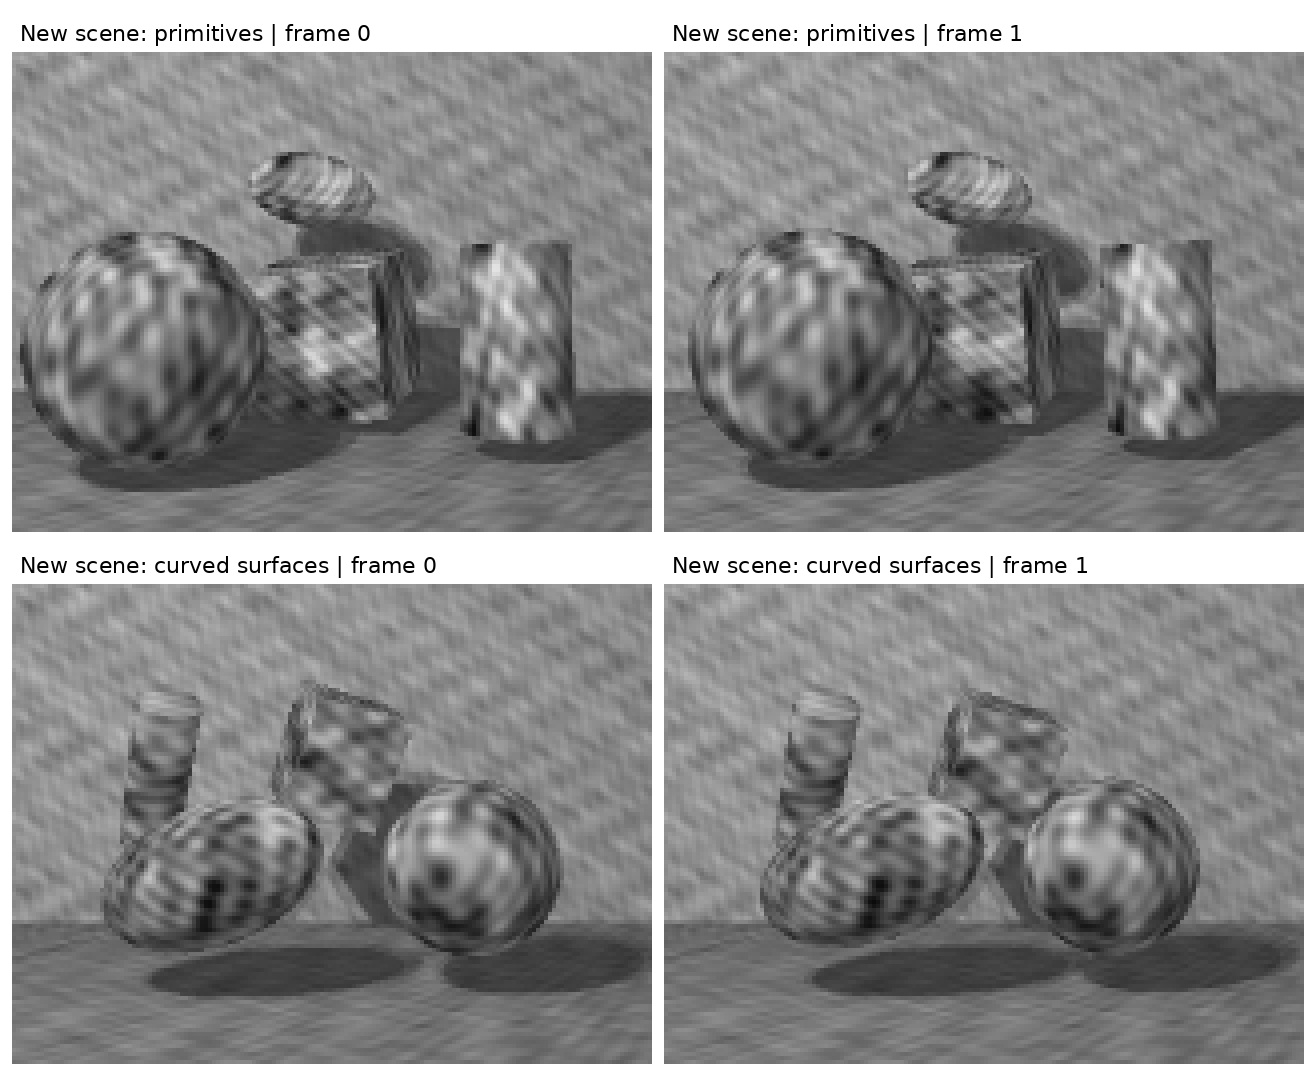
\includegraphics[width=.94\linewidth]{figures/heldout_inputs.png}
\caption{新規条件の入力例。上段は基本配置、下段は曲面配置です。左が時刻0、右が時刻1です。
推定に使用した160$\times$120の灰度を表示しています。表示の拡大は推定解像度の増加ではありません。}
\end{figure}
\begin{figure}[H]\centering
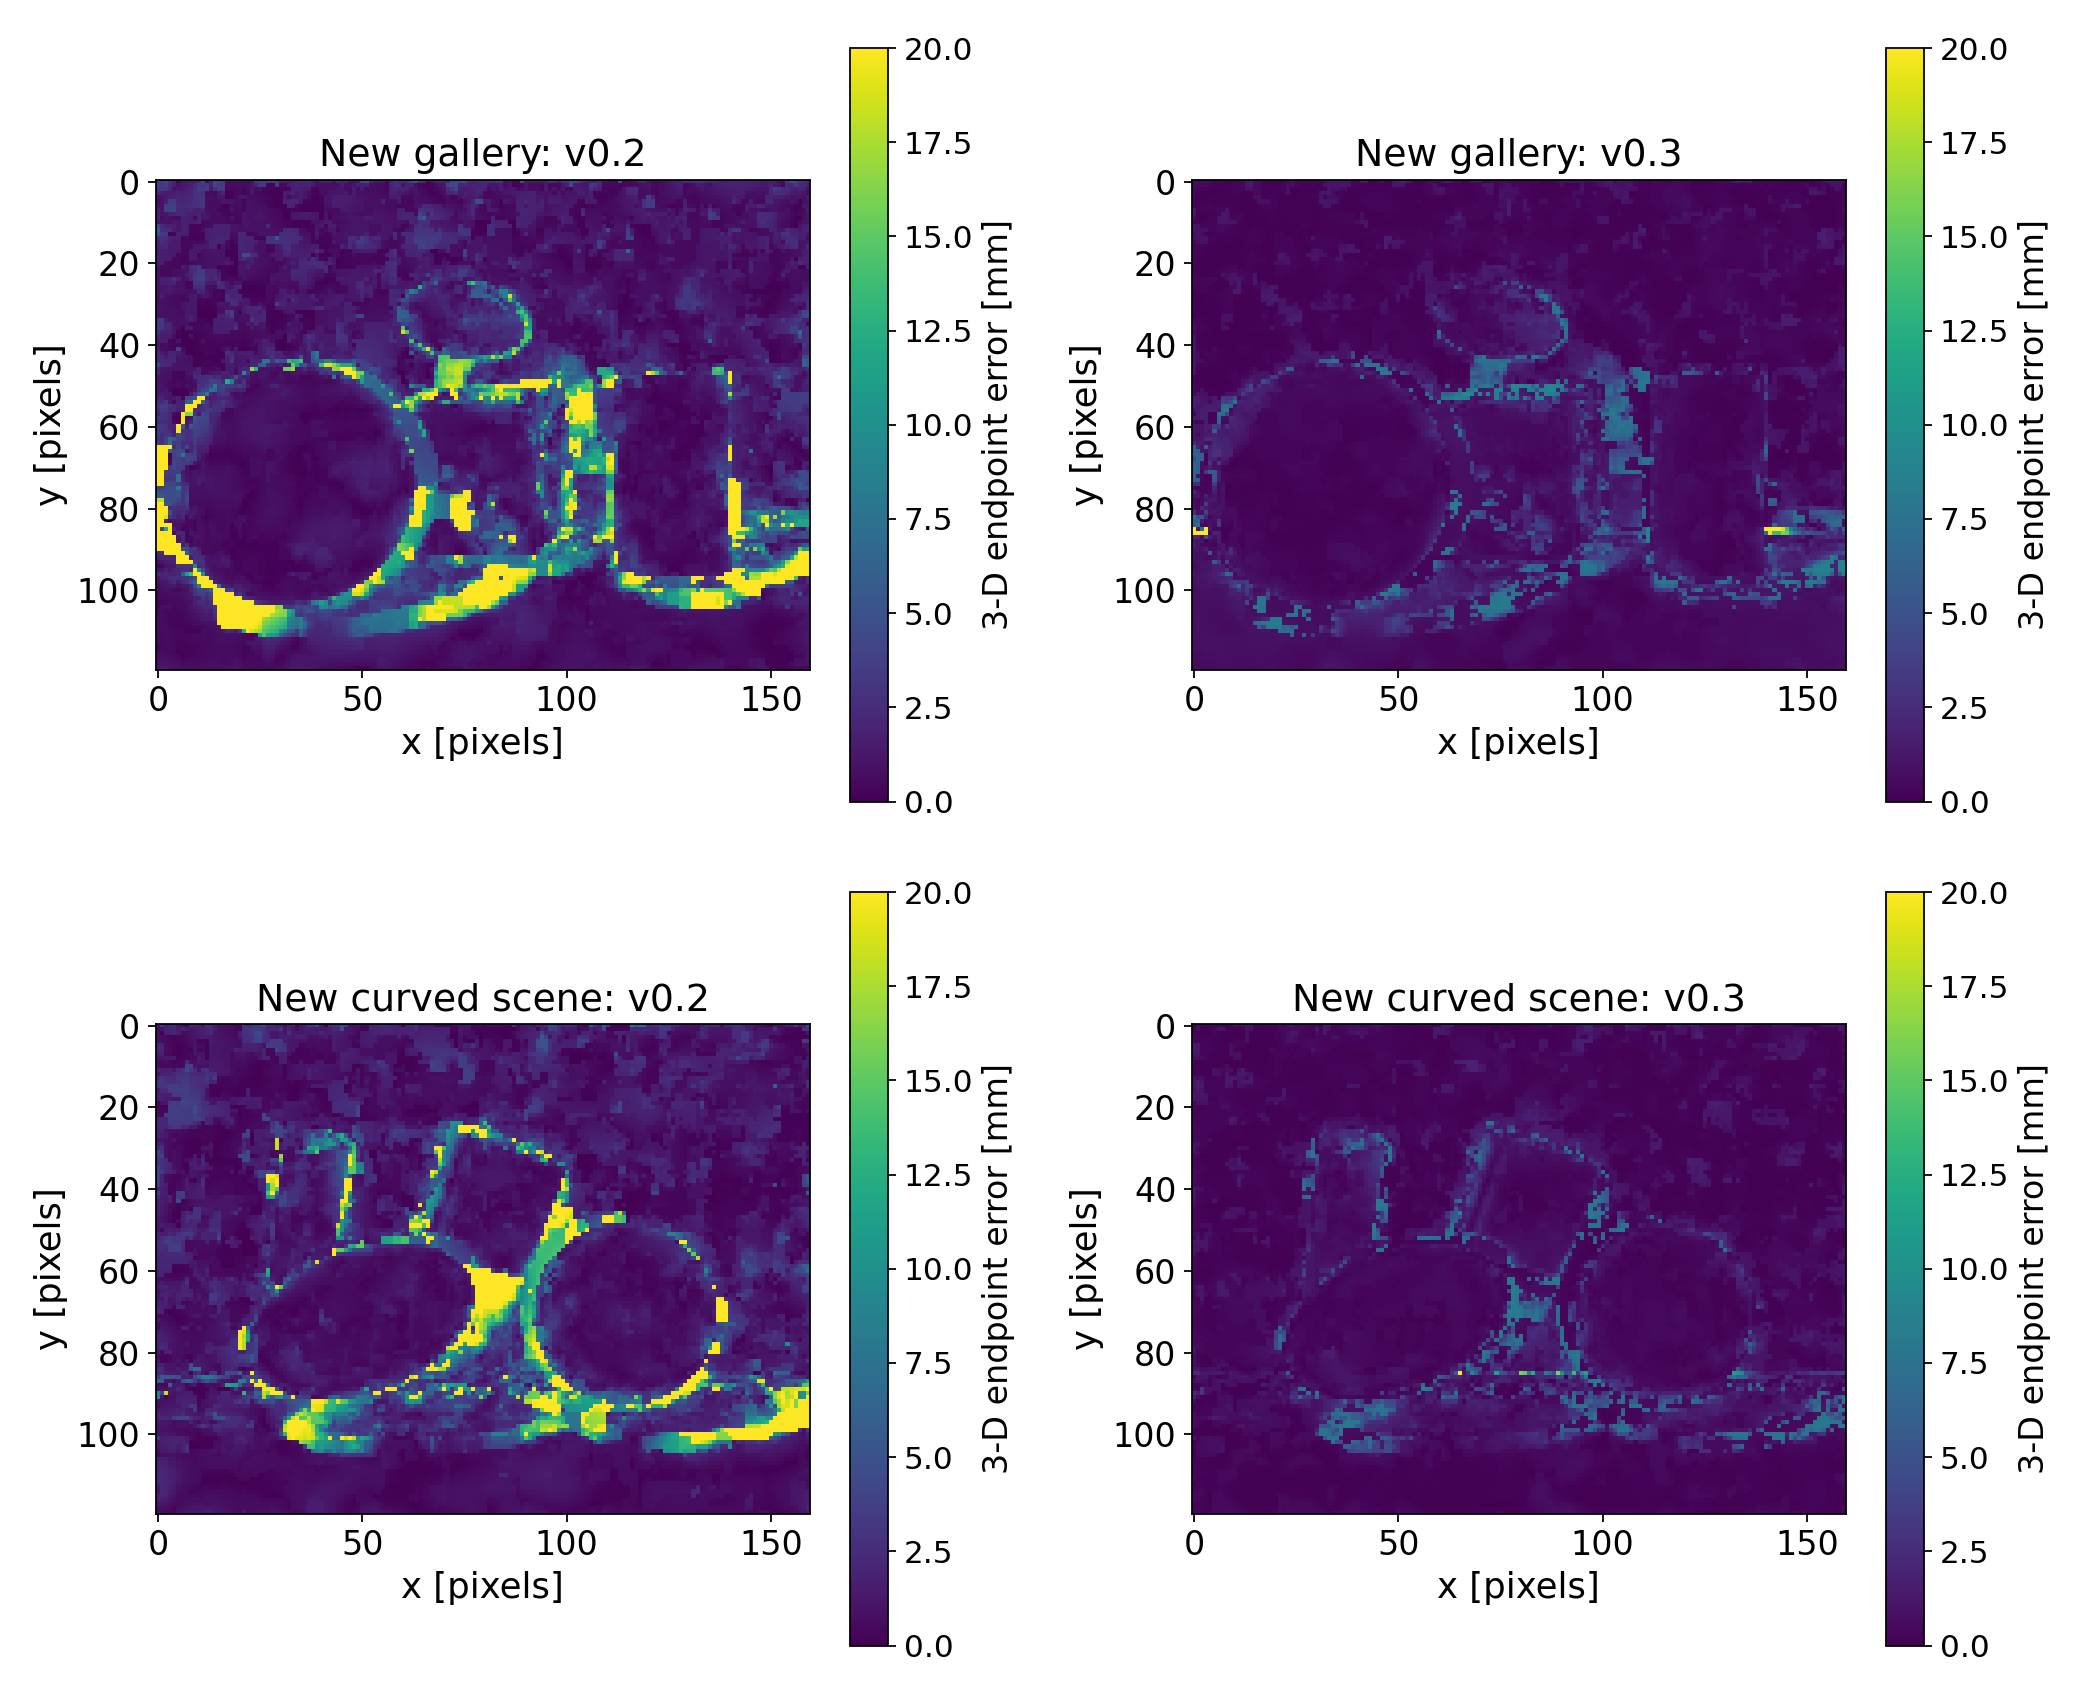
\includegraphics[width=.96\linewidth]{figures/paired_errors.png}
\caption{新規入力での3次元端点誤差。左が第0.2版、右が標準版です。各画像の尺度は同一で、20 mmで表示を飽和させています。
図は遮蔽を含む全画素です。表示上限を超える値も、各評価集合の数値集計から除外していません。}
\end{figure}

\subsection{深度精度・幾何整合性との交換条件}
\begin{table}[H]\centering
\small
\setlength{\tabcolsep}{4pt}
\caption{深度と幾何整合性の変化。全てmm、6入力の平均。変位誤差とは別の指標です。}
\begin{tabular}{llrrr}
\toprule
区分 & 手法 & 時刻0深度RMSE & 時刻1深度RMSE & 幾何残差平均\\\midrule
再試験 & 第0.2版 & 1.862 & 1.888 & 0.204\\
再試験 & 標準版 & 2.088 & 1.973 & 0.460\\
新規条件 & 第0.2版 & 1.811 & 1.853 & 0.203\\
新規条件 & 標準版 & 1.976 & 1.911 & 0.419\\
\bottomrule
\end{tabular}
\end{table}

変位の改善は、全ての出力が同時に改善したという意味ではありません。
新規6入力の深度RMSEは、時刻0で約1.811 mmから1.976 mm、時刻1で1.853 mmから1.911 mmへ増加しました。
支持点の平均幾何残差も約0.203 mmから0.419 mmへ増えています。
悪い対応の幾何拘束をHuber化で弱め、別の運動整合項を用いた結果として、
変位精度と直接の深度・対応整合性の交換条件が生じています。
本版を深度補正だけの評価で前版より優れているとは主張しません。

\subsection{一つずつ外したときの変化}
\begingroup\small
\setlength{\tabcolsep}{4pt}
\begin{longtable}{lrrrrr}
\caption{19構成の同一入力比較。時間以外の単位はmm。基準は「標準版」です。}\\
\toprule
条件 & 共通可視 & 動体 & 静止灰度変化 & 遮蔽 & 時間 [s]\\\midrule\endfirsthead
\toprule
条件 & 共通可視 & 動体 & 静止灰度変化 & 遮蔽 & 時間 [s]\\\midrule\endhead
\bottomrule\endfoot
第0.2版 & 3.253 & 2.552 & 22.855 & 15.554 & 34.392\\
標準版 & 0.913 & 0.978 & 3.266 & 2.395 & 9.817\\
剛体補助項なし & 3.148 & 2.525 & 21.183 & 13.830 & 9.648\\
幾何を二乗に戻す & 1.250 & 1.143 & 7.967 & 4.178 & 9.651\\
剛体なし・幾何二乗 & 3.148 & 2.525 & 21.183 & 13.830 & 9.890\\
恒等候補の予約なし & 0.940 & 0.976 & 4.101 & 2.396 & 10.072\\
全探索 & 0.926 & 0.965 & 3.490 & 2.940 & 22.982\\
双対を毎回初期化 & 0.667 & 0.723 & 2.437 & 2.303 & 10.013\\
計算融合なし & 0.913 & 0.978 & 3.266 & 2.395 & 10.324\\
長反復 & 0.917 & 0.988 & 3.120 & 2.388 & 24.277\\
短反復 & 0.846 & 0.922 & 3.370 & 2.393 & 7.283\\
一次TV & 0.922 & 1.028 & 3.255 & 2.409 & 6.524\\
輝度利得補正あり & 1.031 & 0.897 & 2.252 & 1.737 & 10.128\\
移動上限なし & 0.706 & 0.707 & 0.561 & 30.640 & 19.362\\
正則化の境界停止なし & 0.910 & 0.991 & 3.256 & 3.271 & 10.042\\
往復照合なし & 1.251 & 1.333 & 5.110 & 7.800 & 8.499\\
弱い剛体補助項 & 1.752 & 1.587 & 11.106 & 5.323 & 9.460\\
ステップ比4 & 0.785 & 0.818 & 3.587 & 2.356 & 10.103\\
同値な計算核変更のみ & 3.253 & 2.552 & 22.855 & 15.554 & 32.593\\
\end{longtable}
\endgroup

表の各値は同じ基本配置・雑音種37での測定です。一条件の比較だけから普遍的な優位性を主張しません。
「境界停止なし」は正則化だけの変更であり、候補の段差検査と剛体領域の構築は残ります。
「上限なし」は候補の物理検査と変位球の両方を外しますが、計算上の最大探索半径は残ります。
「剛体なし」でも恒等候補は選択肢として残り、静止を強制しません。

この入力では、双対を毎回ゼロに戻す構成が標準版より低い変位誤差を示しました。
一方、標準版より大きな固定点残差を持ち、解の最適性が高いと解釈することはできません。
短反復版や一次TVも、時間と誤差の観点で有力な構成でした。
事前に固定した標準構成を新規入力の結果に合わせて選び直さず、これらを探索的な結果として分けて示します。

\subsection{組合せによる効果}
\begin{table}[H]\centering
\small
\setlength{\tabcolsep}{4pt}
\caption{幾何Huber化と剛体補助項の2×2比較。差の差は相互作用の記述値です。}
\begin{tabular}{llrrr}
\toprule
Huber & 剛体補助項 & 共通可視 [mm] & 動体 [mm] & 静止灰度変化 [mm]\\\midrule
0 & 0 & 3.148 & 2.525 & 21.183\\
1 & 0 & 3.148 & 2.525 & 21.183\\
0 & 1 & 1.250 & 1.143 & 7.967\\
1 & 1 & 0.913 & 0.978 & 3.266\\
差の差 &  & -0.337 & -0.164 & -4.700\\
\bottomrule
\end{tabular}
\end{table}

Huber化が単独で効くか、剛体補助項が存在するときに効くかを分離するため、
両因子を同じ入力で交差させました。
$E_{hr}$をHuberの有無$h$、剛体補助項の有無$r$に対する誤差とすると、
相互作用の差は$E_{11}-E_{01}-E_{10}+E_{00}$です。
これはこの条件での誤差の差であり、独立な多数のシーンに対する統計的な交互作用検定ではありません。

\subsection{速度、最適化誤差、反復数}
\begin{table}[H]\centering
\small
\setlength{\tabcolsep}{4pt}
\caption{C++処理時間の内訳。全て秒。「残り」は作用素の構築・最適化・出力を含みます。}
\begin{tabular}{lrrrrr}
\toprule
条件 & 対応探索 & 補助項 & 残り & 合計 [s] & 内側反復\\\midrule
第0.2版 & 19.11 & 0.000 & 15.28 & 34.39 & 1800\\
同値な計算核変更のみ & 17.39 & 0.000 & 15.21 & 32.59 & 1800\\
標準版 & 3.57 & 0.004 & 6.24 & 9.82 & 700\\
全探索 & 16.40 & 0.003 & 6.58 & 22.98 & 700\\
計算融合なし & 3.63 & 0.003 & 6.69 & 10.32 & 700\\
双対を毎回初期化 & 3.72 & 0.003 & 6.29 & 10.01 & 700\\
短反復 & 3.67 & 0.003 & 3.61 & 7.28 & 400\\
長反復 & 3.72 & 0.003 & 20.56 & 24.28 & 2400\\
\bottomrule
\end{tabular}
\end{table}

候補削減は離散問題を変えますが、計算融合は同じ反復式を計算する実装変更です。
双対初期値の再利用と反復数削減は、同じ目的関数でも有限時間の到達点を変え得ます。
これらをひとまとめに「同じ解をそのまま高速に計算した」とは記述しません。
\begin{figure}[H]\centering
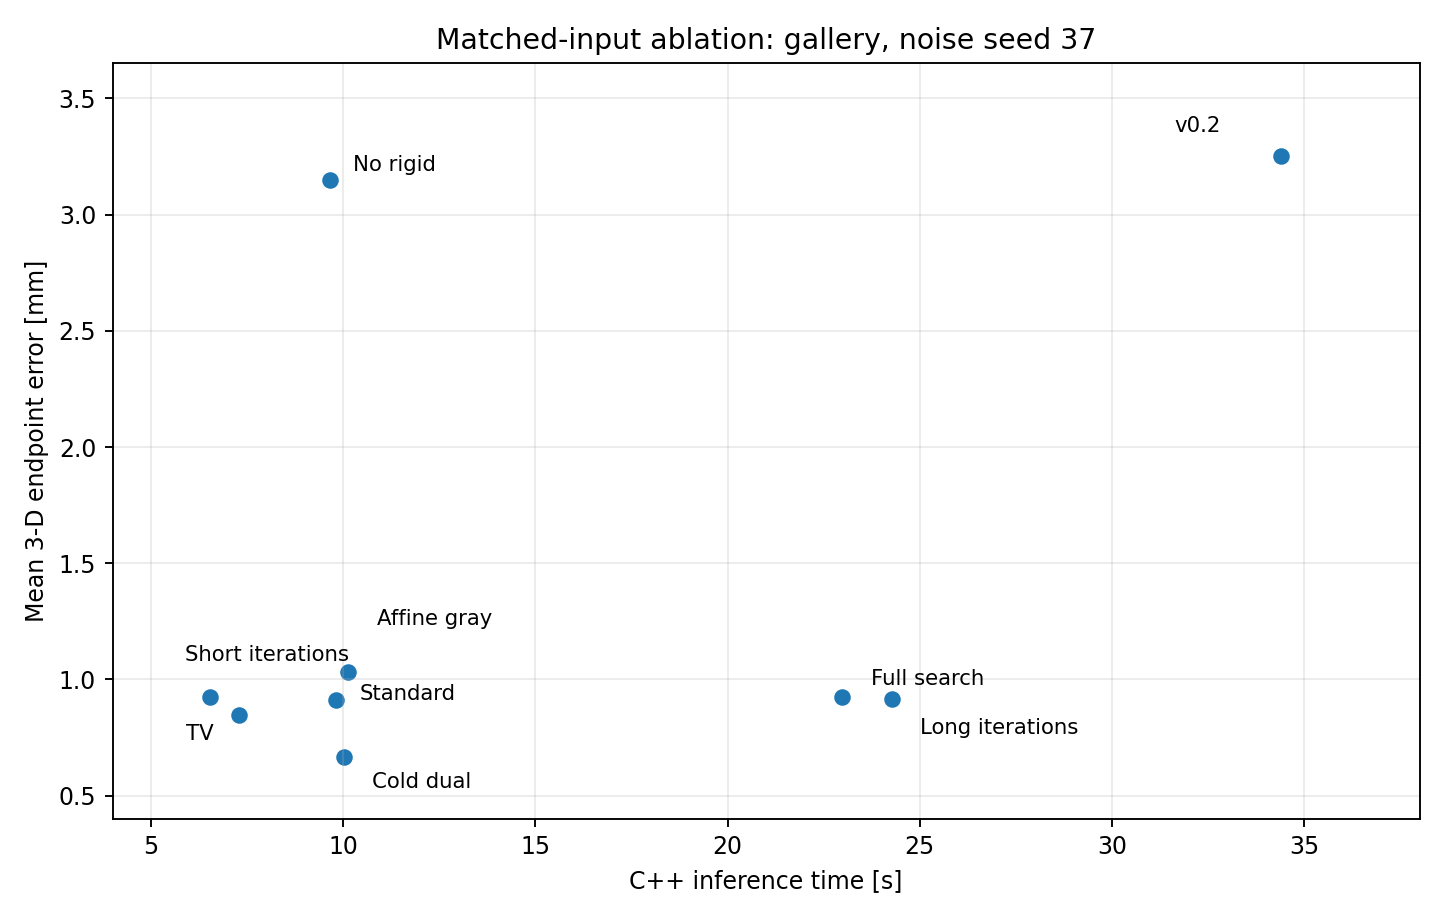
\includegraphics[width=.9\linewidth]{figures/speed_accuracy.png}
\caption{アブレーション入力での速度と精度。横軸はC++処理時間、縦軸は3次元端点誤差です。
左下ほどこの条件では有利ですが、長い反復による目的値低下が正解誤差の低下と一致するとは限りません。}
\end{figure}
\begin{table}[H]\centering
\small
\setlength{\tabcolsep}{4pt}
\caption{同じ形式の目的関数の到達値と固定点残差。候補の選択は変わり得ます。}
\begin{tabular}{lrrrr}
\toprule
条件 & 最終保持目的値 & $r_P$ & $r_D$ & 誤差 [mm]\\\midrule
標準版 & 75049.59 & 0.02105 & 0.32530 & 0.913\\
短反復 & 74400.30 & 0.06550 & 0.48735 & 0.846\\
長反復 & 74904.98 & 0.00388 & 0.03734 & 0.917\\
双対を毎回初期化 & 75150.42 & 0.20814 & 0.39200 & 0.667\\
ステップ比4 & 76275.29 & 0.03285 & 0.87767 & 0.785\\
\bottomrule
\end{tabular}
\end{table}

長反復版と標準版の比較は、精度指標だけでなく最終目的値と固定点残差も確認します。
異なる正則化や支持を持つ手法間では目的関数自体が異なるので、目的値の大小を性能順位には使いません。

\section{反例・失敗条件}
\begingroup\small
\setlength{\tabcolsep}{4pt}
\begin{longtable}{llrrrr}
\caption{ストレス条件と反例。誤差単位はmm。各条件は1入力で、信頼区間ではありません。}\\
\toprule
条件 & 手法 & 共通可視 & 動体 & 遮蔽 & 時間 [s]\\\midrule\endfirsthead
\toprule
条件 & 手法 & 共通可視 & 動体 & 遮蔽 & 時間 [s]\\\midrule\endhead
\bottomrule\endfoot
同深度・独立運動 & 標準版 & 0.961 & 2.459 & 3.665 & 9.94\\
同深度・独立運動 & 剛体補助項なし & 2.181 & 1.019 & 13.733 & 9.43\\
同深度・独立運動 & 輝度利得補正あり & 1.291 & 2.880 & 3.556 & 9.77\\
照明差 & 標準版 & 1.337 & 0.979 & 2.509 & 10.06\\
照明差 & 剛体補助項なし & 3.733 & 2.595 & 13.040 & 9.47\\
照明差 & 輝度利得補正あり & 1.061 & 0.852 & 1.855 & 9.64\\
弱い模様 & 標準版 & 6.104 & 2.344 & 6.661 & 9.62\\
弱い模様 & 剛体補助項なし & 9.491 & 6.564 & 31.107 & 9.60\\
弱い模様 & 輝度利得補正あり & 6.175 & 2.261 & 7.282 & 9.73\\
深度欠測8\% & 標準版 & 1.011 & 1.023 & 5.425 & 8.00\\
深度欠測8\% & 剛体補助項なし & 3.392 & 2.752 & 12.465 & 7.90\\
深度欠測8\% & 輝度利得補正あり & 1.126 & 0.909 & 5.321 & 8.07\\
均一球の回転 & 標準版 & 10.897 & 19.669 & 31.754 & 9.48\\
均一球の回転 & 剛体補助項なし & 11.750 & 19.235 & 32.809 & 8.99\\
均一球の回転 & 輝度利得補正あり & 10.981 & 20.016 & 31.952 & 9.31\\
模様付き球の回転 & 標準版 & 0.586 & 1.157 & 1.352 & 10.58\\
模様付き球の回転 & 剛体補助項なし & 1.496 & 2.270 & 3.607 & 10.10\\
模様付き球の回転 & 輝度利得補正あり & 0.860 & 1.155 & 1.626 & 10.20\\
誤った2 cm上限 & 2 cm上限 & 2.361 & 6.547 & 10.168 & 8.06\\
誤った2 cm上限 & 正しい5 cm上限 & 0.806 & 0.764 & 3.701 & 9.49\\
320×240 & 標準版 & 0.586 & 0.533 & 1.121 & 51.17\\
\end{longtable}
\endgroup

\subsection{同一深度の独立運動}
二つの接する有限平面を同じ奥行きへ置き、一方を上、他方を下へそれぞれ12 mm動かします。
時刻0の深度だけでは、その境界で連結成分を分けられません。
一つの剛体変換が両方の運動を十分に表せないため、
採用検査を通った補助項でも偏りを導入することがあります。
この条件は、標準版が全ての入力の動体精度で「剛体なし」を上回るという主張への反例検査です。
残差の中央値が小さいことは、領域の全点が同じ剛体運動を共有する保証ではありません。
実際に、動体誤差は補助項なしの約1.019 mmに対して標準版は約2.459 mmでした。
ただし共通可視領域全体では、静止背景の改善によって標準版が有利に見えます。
このため、動体と静止域を分けた評価が不可欠です。
\begin{figure}[H]\centering
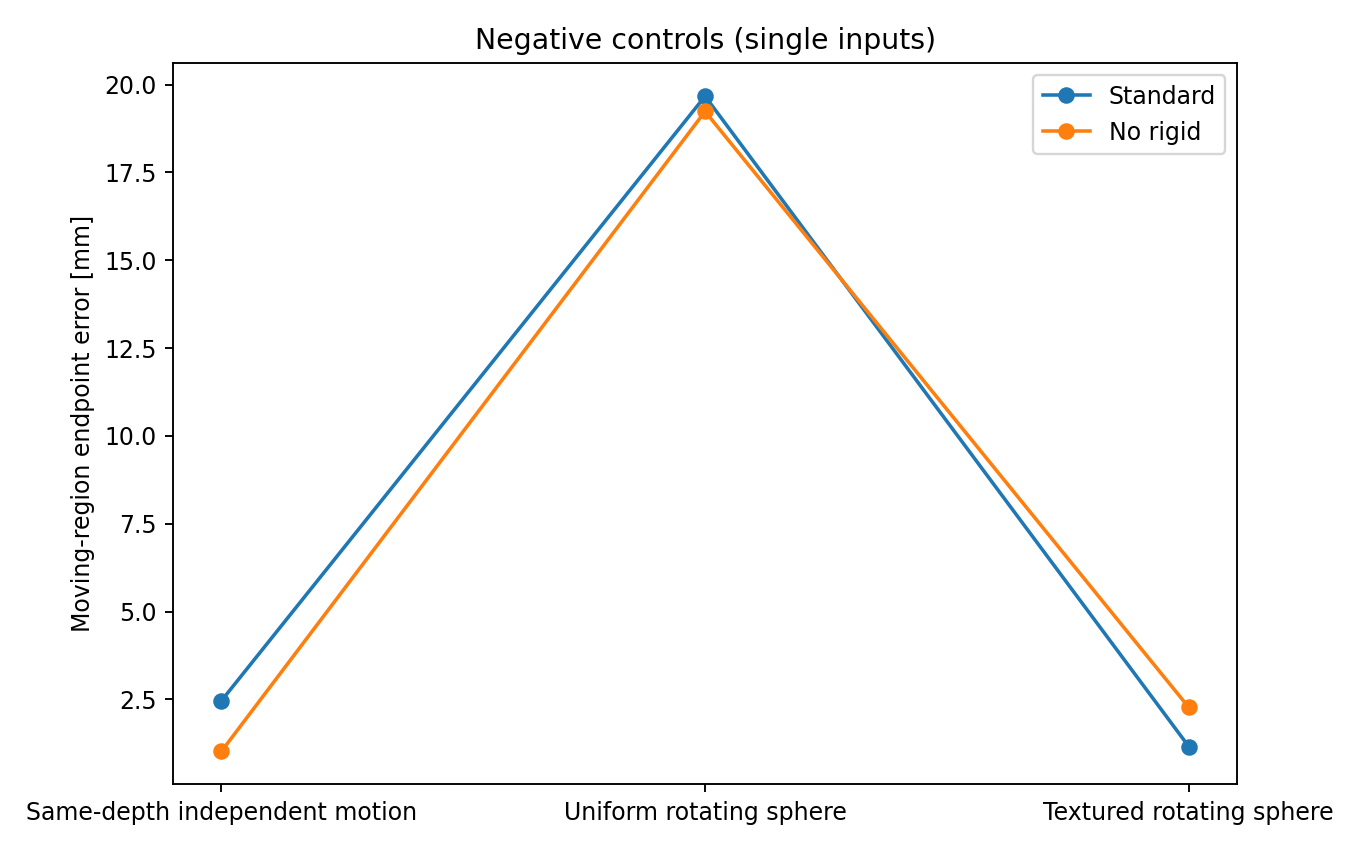
\includegraphics[width=.96\linewidth]{figures/negative_controls.png}
\caption{同一深度の独立運動と、球の回転に対する負の対照。背景を含めず、動体集合だけで誤差を比較しています。}
\end{figure}

\subsection{観測から区別できない運動}
\begin{proposition}[模様のない球の回転]
均一な反射率の球、固定カメラ、固定照明を考えます。中心を変えない球の回転は、
理想的な深度と灰度画像を変えません。一方、球の材料点の変位は一般に0ではありません。
従って、これらの観測と移動上限だけでは材料点のシーンフローを一意に決定できません。
\end{proposition}
\begin{proof}
球の占める集合は中心周りの回転で不変です。各画素で最前面となる位置、世界座標での法線、
均一な反射率も不変なので、深度と灰度は同じです。
同じ材料点$a$の位置は$c+Qa$であり、$Qa\ne a$なら移動します。
十分小さな回転と静止はともに移動上限を満たし、異なる運動が同じ観測を与えます。
\end{proof}
模様を材料座標へ固定すれば観測の手掛かりが増えますが、反復模様や一方向の縞には曖昧さが残ります。
剛体補助項は、存在しない観測情報を新たに作るものではありません。

\subsection{その他の適用限界}
幾何Huber化は、悪い対応に対する力を弱めますが、正しい対応の存在や採用を保証しません。
往復整合が成立する誤対応もあります。照明差の利得補正は局所的なモデルであり、
影の境界、反射、透明物体まで表現するものではありません。

欠測をまたぐ正則化辺は保守的に切るため、深度の穴を埋める実装ではありません。
欠測支持を表示した上で数値配列を返し、支持されない数値を物理的な面として用いないことを入力契約に含めます。

誤った小さな移動上限は、真の解を制約集合から除きます。上限違反が0\%であることは正確性の証明になりません。
固定カメラという仮定が外れる場合は、カメラ運動を補償した共通座標で幾何を定義し直す必要があります。
本実装にはカメラ姿勢の同時推定を含めません。

\section{実装仕様と再現手順}
\subsection{構成と配列契約}
\begin{center}\small
\begin{tabularx}{\linewidth}{lX}\toprule ソース & 責任\\\midrule
\code{cpp/matcher.cpp} & 観測照合、深度区間検査、有限候補、往復支持\\
\code{cpp/rigid.cpp} & 観測深度の連結領域、重み付きHorn法、頑健な補助項\\
\code{cpp/solver.cpp} & 疎行列、転置積、対角前処理、近接写像、外側更新\\
\code{cpp/renderer.cpp} & 基本形状の光線交差、灰度・深度描画\\
\code{cpp/bindings_c.cpp} & C ABI、入力検査、結果の所有権\\
\code{api.py}, \code{_ffi.py} & NumPy入力の整形、ctypes呼び出し、C++配列の複製\\
\code{scripts/benchmark_v03.py} & 固定した比較条件、入力ハッシュ、評価と保存\\
\code{tests/test_v03.py} & 新規核、数値一致、境界、試験条件の検査\\\bottomrule
\end{tabularx}\end{center}
灰度は$H\times W$、深度は$H\times W$、フローは$H\times W\times2$、内部パラメータは
$(f_x,f_y,c_x,c_y)$です。入力画像は有限の$[0,1]$、深度欠測はNaNまたは非正値で表します。
戻り値はC++所有者を解放する前に複製し、外部から解放済みメモリを参照しません。

出力の\code{support}は前処理の支持、\code{rigid_weight}は補助項の重み、
\code{components}は観測深度の連結番号です。
これらは真の可視性、正答確率、物体番号を意味しません。
\code{initial_scene_flow}は支持された最初の対応の逆投影であり、最適化結果ではありません。

\subsection{環境と実行}
通常のオンライン環境の入口は以下です。
\begin{lstlisting}
uv sync
uv run python scripts/build_baseline.py
uv run python -m pytest -q
uv run python scripts/benchmark_v03.py --part all
uv run python scripts/report_v03.py
cd docs/v03
lualatex -interaction=nonstopmode -halt-on-error theory_ja.tex
lualatex -interaction=nonstopmode -halt-on-error theory_ja.tex
\end{lstlisting}
今回の実行環境は外部への依存パッケージ取得に失敗したため、uvで作った環境から既存の依存を再利用しました。
\code{uv pip install --no-build-isolation --no-deps -e .}による導入とビルドを確認しています。
新規ダウンロードを伴う\code{uv sync}、および依存解決済み\code{uv.lock}の生成まで検証したとはしません。
uvのロックと同期の意味は公式文書\cite{uv}を参照しています。
実行した版は\code{requirements-verified.txt}と環境JSONへ記録します。

\subsection{検証の範囲}
\begin{table}[H]\centering
\small
\setlength{\tabcolsep}{4pt}
\caption{実行した数値検査。小さい差はこの環境の丸め誤差の範囲です。}
\begin{tabular}{p{.68\linewidth}r}
\toprule
検査項目 & 結果\\\midrule
保存配列の制約検査 & 70組\\
移動上限の最大超過 [m] & 1.39e-17\\
深度許容域の最大超過 [m] & 2.32e-16\\
再投影フローの最大差 [画素] & 0.00e+00\\
融合あり／なしの変位最大差 [m] & 1.25e-16\\
同値核変更／前版の変位最大差 [m] & 0.00e+00\\
展開・再ビルド後の自動試験 & 94 passed in 7.95s\\
再計算した代表入力の最大配列差 & 0.000000000000\\
\bottomrule
\end{tabular}
\end{table}

旧評価関数の\code{max_estimated_motion_mm}がメートル値を保存していた単位不備も修正し、保存変位からmmへ再集計しました。端点誤差と処理時間には影響しません。

単位四元数による回転推定は、平面・非平面の点集合と複数の回転角で検査します。
双対Huber近接写像は閉形式と比較し、融合あり／なしで出力を照合します。
移動球、深度許容域、再投影、転置の随伴関係、外側の最良目的値の非増加、
反復数の計数、無効設定、欠測支持、生成器の移動上限を検査します。
これらは試験した条件での検査であって、任意のコンパイラ・全入力への形式検証ではありません。

\section{結論}
本版は、対応候補を減らす近似、計算式を変えない実装最適化、反復の再利用、
そして運動に関する仮定を加えるモデル変更を区別しました。
精度向上を一つの数値だけで示すのではなく、同一入力の新旧比較、新規条件、
単一要素除去、因子の組合せ、剛体仮定の反例で確かめます。

本研究の到達点は、境界を保ちつつ有限の移動上限を課すC++補正器について、
動作する数学的仕様と測定結果を対応付けたことです。
モデルが適合する人工データでの改善と、情報不足や誤った仮定による失敗を同時に示し、
実データ・欠測補完・実時間処理を達成済みとみなさないことが重要です。

\appendix
\section{重み付きHorn法の具体式}
本付録の点$x_i,y_i$、重心$c_x,c_y$、行列$H,N$、四元数$q$、重み総和$W$は、
以下で定義する剛体最小二乗の局所記号です。本文の画像サイズ・内部パラメータ・対応座標とは区別します。
重み$w_i\ge0$、総和$W>0$に対して、出発点$x_i$と到着点$y_i$の重み付き重心を$c_x,c_y$とします。
交差行列を$H=\sum_i w_i(x_i-c_x)(y_i-c_y)^\T$と置き、$H_{ij}$をその要素とします。
\begin{equation}
N=\begin{pmatrix}
\operatorname{tr}H&H_{23}-H_{32}&H_{31}-H_{13}&H_{12}-H_{21}\\
H_{23}-H_{32}&H_{11}-H_{22}-H_{33}&H_{12}+H_{21}&H_{13}+H_{31}\\
H_{31}-H_{13}&H_{12}+H_{21}&-H_{11}+H_{22}-H_{33}&H_{23}+H_{32}\\
H_{12}-H_{21}&H_{13}+H_{31}&H_{23}+H_{32}&-H_{11}-H_{22}+H_{33}
\end{pmatrix}
\end{equation}
最大の\textbf{代数的}固有値に対応する単位固有ベクトルを$q=(a,b,c,d)^\T$とします。
最大絶対値の固有値ではありません。回転は
\begin{equation}
Q=\begin{pmatrix}
a^2+b^2-c^2-d^2&2(bc-ad)&2(bd+ac)\\
2(bc+ad)&a^2-b^2+c^2-d^2&2(cd-ab)\\
2(bd-ac)&2(cd+ab)&a^2-b^2-c^2+d^2
\end{pmatrix},\quad t=c_y-Qc_x
\end{equation}
です。これが重み付き剛体最小二乗を解く理由は、重心を引いた二乗誤差の可変部分が
$-2\operatorname{tr}(QH)$となり、四元数表示で$-2q^\T Nq$となるためです。
単位球上の二次形式の最大値は最大代数固有値です\cite{horn}。
実装は4次の対称Jacobi法を最大64回用い、最大非対角要素が
$10^{-14}\max(1,|\operatorname{tr}H|)$未満で終了します。

\section{標準パラメータ一覧}
\begingroup\small
\setlength{\tabcolsep}{4pt}
\begin{longtable}{lll}
\caption{標準Configの全46項目。数値配列の並びもこの順序です。}\\
\toprule
設定 & 値 & 意味\\\midrule\endfirsthead
\toprule
設定 & 値 & 意味\\\midrule\endhead
\bottomrule\endfoot
\code{scale} & 0.01 & 長さの無次元化尺度 [m]\\
\code{sigma_depth} & 0.003 & 深度の公称誤差 [m]\\
\code{sigma_flow} & 0.7 & フロー誤差 [画素]\\
\code{sigma_image} & 0.025 & 灰度残差尺度\\
\code{sigma_geometry} & 0.0008 & 幾何残差尺度 [m]\\
\code{max_motion} & 0.05 & 移動距離の上限 [m]\\
\code{trust_sigma} & 4.0 & 深度補正幅の倍率\\
\code{min_depth} & 0.1 & 最小深度 [m]\\
\code{max_depth} & 5.0 & 最大深度 [m]\\
\code{edge_threshold} & 0.06 & 深度段差の閾値 [m]\\
\code{depth_alpha1} & 1.2 & 深度の一次残差係数\\
\code{depth_alpha0} & 4.0 & 深度の二階係数\\
\code{flow_alpha1} & 2.0 & 変位の一次残差係数\\
\code{flow_alpha0} & 6.0 & 変位の二階係数\\
\code{image_weight} & 1.0 & 画像照合の係数\\
\code{flow_weight} & 0.025 & 初期フロー整合の係数\\
\code{flow_truncation} & 9.0 & 初期フロー損失の切断値\\
\code{photo_reject} & 3.0 & 画像照合の採用上限\\
\code{huber_k} & 3.0 & 深度Huberの折れ点\\
\code{ridge} & 1e-06 & 補助場の二次項係数\\
\code{iterations} & 400 & 最初の内側反復数\\
\code{outer_iterations} & 3 & 外側の反復数\\
\code{candidate_count} & 24 & 保持候補数\\
\code{max_search} & 18 & 探索半径の計算上限 [画素]\\
\code{patch_radius} & 2 & 画像窓の半径 [画素]\\
\code{edge_aware} & True & 正則化の境界停止\\
\code{use_tgv} & True & 二階正則化（偽なら一次TV）\\
\code{enforce_bound} & True & 候補・変位の物理制約\\
\code{centered_photo} & True & 平均輝度差の除去\\
\code{reciprocal_check} & True & 往復照合\\
\code{diverse_candidates} & True & 候補間隔による多様化\\
\code{fast_match} & True & 階層的な有限探索\\
\code{affine_photo} & False & 輝度利得の代入型補正\\
\code{rigid_prior} & True & 観測由来の剛体補助項\\
\code{fused_solver} & True & 双対計算の融合\\
\code{warm_start} & True & 双対初期値の再利用\\
\code{keep_identity} & True & 恒等候補の保持\\
\code{later_iterations} & 150 & 2回目以降の内側反復数\\
\code{coarse_stride} & 2 & 整数探索の間隔\\
\code{seed_count} & 3 & 小数画素探索の種の数\\
\code{rigid_min_points} & 24 & 剛体推定の最小対応数\\
\code{rigid_sigma} & 0.0015 & 剛体補助項の尺度 [m]\\
\code{rigid_huber} & 0.006 & 剛体IRLSの折れ点 [m]\\
\code{step_balance} & 1.0 & 主双対ステップの相反倍率\\
\code{geometry_huber} & True & ベクトル幾何Huber\\
\code{geometry_k} & 3.0 & 幾何Huberの折れ点\\
\end{longtable}
\endgroup

\section{文書の読み方とスタイル上の変更}
前版の実験経緯中心の構成から、入力契約、演算子、目的関数、解法、保証、実験、失敗条件という順序へ改めました。
数式の記号は初出時に定義し、同じ記号を異なる目的に使わないようにしています。
焦点距離とフロー成分のように混同が起こる式では、局所的に明示した添字を使います。
定理に近い主張には仮定と証明を付け、実験上の傾向を数学的保証として扱いません。

各図表の説明には単位、評価集合、比較条件、表示尺度を含めます。
数値は保存JSONから自動生成し、本文の転記によりCSVと食い違うことを避けます。
速度は計測対象を、誤差棒は何のばらつきかを記します。
これらの編集方針はIEEEの数式・引用の指針\cite{ieee}と、
NeurIPSの仮定・再現性・限界・計算量・誤差棒に関する検査項目\cite{checklist}に基づきます。
本資料は特定の学会へ投稿済み、査読済み、または外部認証済みというものではありません。

\begin{thebibliography}{99}\small
\bibitem{yao} Y. Yao, M. Roxas, R. Ishikawa, S. Ando, J. Shimamura, T. Oishi.
\emph{Discontinuous and Smooth Depth Completion with Binary Anisotropic Diffusion Tensor}. arXiv:2006.14374, 2020.
\bibitem{dis} T. Kroeger, R. Timofte, D. Dai, L. Van Gool.
\emph{Fast Optical Flow Using Dense Inverse Search}. ECCV, 2016. arXiv:1603.03590.
\bibitem{unflow} S. Meister, J. Hur, S. Roth.
\emph{UnFlow: Unsupervised Learning of Optical Flow with a Bidirectional Census Loss}. AAAI, pp.7251--7259, 2018. arXiv:1711.07837.
\bibitem{vogel} C. Vogel, K. Schindler, S. Roth.
\emph{Piecewise Rigid Scene Flow}. ICCV, 2013. DOI:10.1109/ICCV.2013.174.
\bibitem{horn} B. K. P. Horn.
\emph{Closed-form solution of absolute orientation using unit quaternions}. JOSA A, 4(4), pp.629--642, 1987. DOI:10.1364/JOSAA.4.000629.
\bibitem{pock} T. Pock, A. Chambolle.
\emph{Diagonal preconditioning for first order primal-dual algorithms in convex optimization}. ICCV, pp.1762--1769, 2011. DOI:10.1109/ICCV.2011.6126441.
\bibitem{naganuma} K. Naganuma, S. Ono.
\emph{Variable-Wise Diagonal Preconditioning for Primal-Dual Splitting: Design and Applications}. IEEE Transactions on Signal Processing, 2023. DOI:10.1109/TSP.2023.3304789. arXiv:2301.08468v4.
\bibitem{ieee} IEEE Author Center. \emph{IEEE Editorial Style Manual}.
\url{https://journals.ieeeauthorcenter.ieee.org/your-role-in-article-production/ieee-editorial-style-manual/}. 2026年10月13日確認.
\bibitem{checklist} NeurIPS. \emph{Paper Checklist Guidelines}.
\url{https://neurips.cc/public/guides/PaperChecklist}. 2026年10月13日確認.
\bibitem{uv} Astral. \emph{uv: Locking and syncing}.
\url{https://docs.astral.sh/uv/concepts/projects/sync/}. 2026年10月13日確認.
\end{thebibliography}
\end{document}
